\documentclass[conference]{IEEEtran}
\IEEEoverridecommandlockouts
\usepackage{cite}
\usepackage{cancel}
\usepackage{amsmath,amssymb,amsfonts}
\usepackage{algorithmic}
\usepackage{siunitx}
\usepackage{graphicx}
\usepackage{float}
\usepackage{tikz}
\graphicspath{{images/}}
\usepackage{textcomp}
\def\BibTeX{{\rm B\kern-.05em{\sc i\kern-.025em b}\kern-.08em
    T\kern-.1667em\lower.7ex\hbox{E}\kern-.125emX}}
\begin{document}

\title{Segregating Robots That Do Not Compute}

\author{\IEEEauthorblockN{Jordan Burklund}
\IEEEauthorblockA{\textit{Worcester Polytechnic Institute} \\
Worcester, MA \\
jsburklund@wpi.edu}
\and
\IEEEauthorblockN{Michael Giancola}
\IEEEauthorblockA{\textit{Worcester Polytechnic Institute} \\
Worcester, MA \\
mjgiancola@wpi.edu}
\and
\IEEEauthorblockN{Peter Mitrano}
\IEEEauthorblockA{\textit{Worcester Polytechnic Institute} \\
Worcester, MA \\
pdmitrano@wpi.edu}
}

\maketitle

\begin{abstract}
  In this paper, we reproduce robot aggregation behavior from \cite{gauci_self-organized_2014} on a swarm of simulated robots. We then extend the controller to perform $n$-class segregation. We evolve controllers for this behavior with a genetic algorithm and perform a grid search over all parameters to understand the full parameter space. We find the robust segregation is possible, although not guaranteed. Instead, we prove only that one or two kin-robots executing our controller will aggregate.
\end{abstract}

\begin{IEEEkeywords}
  swarm robotics, robot aggregation, robot segregation
\end{IEEEkeywords}

\section{Introduction and Related Work}
  Several of the methods proposed have demonstrated the ability to aggregate robots and objects in a distributed way, and some have shown the ability to perform such tasks with limited computation and sensing capabilities. Decentralized aggregation is frequently posed as a precursor to other swarm behaviors such as sorting heterogeneous robots for task allocation \cite{gauci_evolving_2014} \cite{dorigo_evolving_2004}. By aggregating, agents can cooperate on tasks, share information, and other higher level swarm behaviors. In nature, we find examples of segregation from cells during embryogenesis to ants sorting their brood \cite{santos_segregation_2014}. We investigate segregating agents into $n$ clusters, so that agents could perform some collective task within their own cluster.

  \subsection{Aggregation and Segregation}
    Robot aggregation is defined as having all robots in the swarm collect at a particular location in a distributed manner. Many swarm aggregation policies require robots to compute bearing and distance to other robots, to sense gradients in the environment, or to otherwise communicate information. However, implementing these communication systems is difficult in practice, so methods that do not require communication or complex sensing are desirable. In \cite{gauci_self-organized_2014}, the authors propose a new class of policies that require no computation.

    The work of \cite{gasparri_swarm_2012} does not restrict itself to a computeless or memoryless solution. Instead they develop an aggregation algorithm which enables robots to respond to guidance commands -- i.e., a human using hand gestures to indicate which direction the swarm should move. They show that swarms running their algorithm are able to follow guidance commands and stay aggregated without colliding. A simpler controller is used in \cite{bahgeci_evolving_2005}, where robots are equipped with IR distance sensors surrounding the robot, 4 microphones, and an omni-directional speaker. The policy is a linear combination of the IR sensor values and the intensity values of the microphones. The authors show that a genetic algorithm is able to find weights for the policy such that robots aggregate together. In \cite{ando_distributed_1999}, the authors present a robot aggregation model with very limited sensing and no memory, but allows the robots to perform computations to determine their next position. They prove that their algorithm is correct in theory, then run the algorithm in simulation.

    Finally, \cite{gauci_self-organized_2014} considers only binary sensor that maps directly to wheel velocities. The authors demonstrate extremely robust aggregation despite these limitations, and they also prove formally that aggregation is guaranteed and find theoretical bounds on aggregation time in simple situations. Similarly, the authors of \cite{gauci_clustering_2014} perform object aggregation with the same restrictions on sensing and control.

    Segregation of robots has received little attention in swarm robotics, however many researchers have focused on sorting of objects \cite{vardy_accelerated_2012} \cite{holland_collective_1998} \cite{tao_wang_collective_2004} \cite{holland_stigmergy_1999}. The study in \cite{santos_segregation_2014} shares our objective, however they assume that each class has the same number of robots and that each robot knows the position of all other robots. In contrast, we adhere to the memoryless computeless controller architecture with a simple ternary sensor. \cite{gros_segregation_2009} also explores segregation robots based on local interactions inspired by gravity, however they require a centralized broadcast or a consensus algorithm to agree on the source or direction of gravity.

  \subsection{Robots That Do Not Compute}

    The memoryless and computeless controllers originally proposed by \cite{gauci_self-organized_2014} has been extended to other tasks and been modified in many ways by other researchers.

    In \cite{kernbach_re-embodiment_2009}, the authors propose an aggregation policy roughly based on observations of bees clustering in an optimal temperature location. In their method, robots are only able to distinguish between collisions between another robot or a wall, can only sense the intensity of a light source when they have collided, and do not communicate information. Although the robots have limited sensing and communication capabilities, the authors show that robots can aggregate to an optimal light intensity location, and that the time to converge to the optimal location improves with increasing number of robots in the environment.

    Robots that do not compute and are memoryless have also been shown to aggregate around a specific object, circle in a ring around an object, and forage for obstacles \cite{johnson_evolving_2016}. In this work, the authors show one can construct simple fitness functions to guide the evolution of controllers to do new yet interesting tasks. However, they also report that in attempting to evolve a controller to rendezvous the robots around an object, they accidentally and consistently evolved a policy where the robots circled around the target object. This demonstrates that designing a fitness function can be hard or unreliable. They achieved rendezvous by initializing the policy at generation zero to the policy found in \cite{gauci_self-organized_2014} for simple aggregation.

\section{Methodology}

  \subsection{Evolving Segregation}

  In order to avoid manually spending time picking parameters or spending tremendous compute time using grid-search time find parameters, we use a simple genetic algorithm to evolve controller parameters. In all our experiments, we use 6 parameters for nothing, kin and non-kin, where each parameter ranges from -1 to 1. In our controller, we then scale this parameter to range from -20cm/s to 20cm/s. We treat aggregation as a special case of 1 class segregation, in which case the final two parameters of the controller are never used. The genetic algorithm we used is unmodified from the example MPGA code provided with the ARGoS simulator. The mutation strategy is simply to mutate each of these 6 parameters with some probability p ($0.05$ in our experiments). If a parameter is selected to be mutated, a uniformly random number from -1 to 1 is picked for the new value. Selection is performed by picking the two most fit individuals (the ones with lowest cost in our formulation), and then forming the next population by crossing the parameters of these two individuals. The original two parents are always kept in the population so that the current fittest individual is never removed until a more fit genome is discovered.

  As with any genetic algorithm, it is important to have a fitness function that accurately assigns cost to behaviors. We explore two different cost functions, and we find that while both of them are intuitive they did not behave as we expected. The first is the cluster metric used by \cite{gauci_self-organized_2014}, which is the proportion of the number of robots in the largest cluster to the total number of robots. we will apply this for each class of robots and sum up the cluster-metric cost for each class to get the total cost.

  We also propose a new cost function to adress some concerns with the cluster metric. The cluster metric described above is problematic because it considers a straight line of robots to be one cluster. In some scenarios, we care about how tightly the swarm is packed in its clusters. Consider the scenario where different classes of swarm robots needs to be collected after a mission, and the must be sorted into clusters so that they can be air-lifted easily. With this scenario in mind, we propose a new metric which uses the centroids of the robots in each class. We borrow the dispersion metric $u^{(t)}$ from \cite{gauci_self-organized_2014}, which essentially computes the sum of distances from each robot to the centroid, but in our case we apply this to each class of robots. Consider $u_i^{(t)}$ to be the dispersion of a particular class $i$ at time $t$. Given all the centroids $\bar{p}_i^{(t)}$ for each class $i$, we call the centroid of all of these centroids $\bar{P}^{(t)}$. We call this the centroid-of-centroids cost function, and it can be defined formally as follows:

  \begin{align*}
  c_{\text{intra}} &= \sum_{i=1}^n u_i^{(t)} \\
  c_{\text{inter}} &= -\frac{1} {4r^2}\sum_{i=1}^n{\lVert \bar{p}_i^{(t)} - \bar{P}_i^{(t)} \rVert}^2 \\
  c_{\text{total}} &=  \sum_{t=0}^{T-1} t (c_{\text{intra}} + c_{\text{intra}}) \\
  \end{align*}

  When we use this cost function in our genetic algorithm, we select fitnessest individuals as those with the lowest cost.


\section{Controller Analysis}

  We found imperially that the parameters [0.5 -0.5 -0.2 0.6 0.6 0.2] successfully achieve segregation. We now analyze this controller formally. First, we prove that a single isolated robot executing this controller will aggregate to a kin robot, or more importantly, a cluster of kin robots. This proof is a variation of the Theorem 5.1 provided in \cite{gauci_self-organized_2014}. Consider a robot situated as shown in Figure \ref{fig:kin_aggregation}. The controller dictates that since a Kin robot is seen, $I=1$, so $v_{l_1} = -0.2$ and $v_{r_1} = 0.6$. This will cause the robot to turn with some radius $R$. Without loss of generality, we define our coordinate system so that $c_i=[0,0]$ with the robot facing the $+x$ axis. For this analysis, we assume that the robot has a fixed, positive inter wheel distance $W$, and that the controller is executed in small finite time steps. Our goal is to show that the distance between the position of the robot after executing our controller for one time step $p'_i$ and the kin robot $p_j$ is less than the distance between the initial position of the robot $p_i$ and the kin robot $p_j$. Formally, this is expressed by the following relationship:

  \begin{figure}[H]
    \centering
    \begin{tikzpicture}
      \draw[white] (-2.25,3.5) rectangle(7.75,-4.75);

      \draw[->] (0,0) -- (7,0);
      \node at (7.2,.2) {x};
      \draw[->] (0,0) -- (0,3);
      \node at (-0.2,3.2) {y};

       % c_i
      \filldraw (0,0) circle (.05);
      \node at (.2,.2) {$c_i$};
      \draw[blue, dashed] (0,0) circle (2);

       % p_i
      \filldraw (0,-2) circle (.05);
      \node at (.2,-2.2) {$p_i$};
      \draw[blue] (0,-2) circle (0.85);
      \node at (-.3,-.8) {$R$};
      \draw[dashed] (0,0) -- (0,-2);

       % p'_i
      \filldraw (1.41,-1.41) circle (.05);
      \node at (1.85,-1.25) {$p'_i$};
      \draw[blue] (1.41,-1.41) circle (0.85);
      \draw[dashed] (0,0) -- (1.41,-1.41);
      \node at (.8,-.3) {$R$};

       % p_j
      \filldraw (5,-3.25) circle (.05);
      \node at (5.2,-3.5) {$p_j$};
      \draw[red] (5,-3.25) circle (1.25);
      \draw (5,-3.25) -- (5,-2);
      \node at (5.3,-2.625) {$r_j$};

      % delta
      \draw[blue] (0,-2) -- (5,-2);
      \draw[blue] (1.41,-1.41) -- (5.3,-2.03);
      \node at (2.5, -2.2) {$\delta$};

      % theta
      \draw (0,-.7) arc [radius=.7, start angle=-90, end angle=-45];
      \node at (.36,-.85) {$\theta$};
    \end{tikzpicture}
    \caption{The robot will always move closer to its Kin.}
    \label{fig:kin_aggregation}
  \end{figure}

  \begin{equation} \label{eq:agg}
    \lVert p_j - p'_i \rVert < \lVert p_j - p_i \rVert
  \end{equation}

  We emphasize that $r_j$ could be the radius of a single kin robot or the radius of a large cluster of kin robots. With this coordinate system and assumptions stated, we can define the coordinate of $p_i$, $p_j$, and $p'_i$.

  \begin{equation}
    \begin{split}
      p_i = \begin{bmatrix}0 \\ -R\end{bmatrix} \\
      p_j = \begin{bmatrix}\delta \\ -(R+r_j)\end{bmatrix} \\
      p'_i = \begin{bmatrix}R\sin(\theta) \\ -R\cos(\theta)\end{bmatrix}
    \end{split}
  \end{equation}

  We then substitute these variables into our inequality (Equation \ref{eq:agg}), and the result is shown in Equation \ref{eq:agg_result}. For the full derivation, see Appendix \ref{thm:1}. In short, the distance of the robot to its kin is guaranteed to decrease until a point where the sensor ray distance $\delta$ is not greater than some simple function of $\theta$ and $R$. We can further calculate exactly how much closer the robot $i$ will be to robot $j$ after executing the $I=1$ state for one time step. As we show in Appendix \ref{thm:2}, the change in distance between the robots is equal to
  $$2R\big((r_j + R)(1 - \cos(\theta))-\delta\sin(\theta)\big)$$
  In both of these equations the dependant variables $\theta$ and $R$ are themselves a function of the inter wheel diameter $W$ and the wheels speeds of the controller $v_{l_1}$ and $v_{l_1}$, which are shown in Equation \ref{eq:theta_and_r}.

  \begin{equation} \label{eq:agg_result}
    \delta > (R + r_j)\tan\bigg(\frac{\theta}{2}\bigg)
  \end{equation}

  \begin{align}
    \begin{split} \label{eq:theta_and_r}
      \theta &= \Delta t\omega = \Delta t \frac{v_{r_1} - v_{l_1}}{W} = \Delta t \frac{0.6 - (-0.2)}{W} = \frac{0.8\Delta t}{W} \\
      R &= \frac{W}{2}\bigg(\frac{v_{r_1} + v_{l_1}}{v_{r_1} - v_{l_1}}\bigg) = \frac{W}{2}\bigg(\frac{0.6 + (-0.2)}{0.6 - (-0.2)}\bigg) = \frac{W}{4}
    \end{split}
  \end{align}

  Combining \ref{eq:theta_and_r} with \ref{eq:agg_result}, we get a useful expression that tells us the conditions under which aggregation is guaranteed (\ref{eq:agg_final_result}). We emphasize that this does not mean aggregation to a kin is guaranteed for all values of $\Delta t$, $r_j$, and $W$. For example, if $\Delta t$ is increased to \SI{1}{\second} then aggregation is likely not guaranteed. We can also determine exactly how much closer the robots get each time, and since this is a function of $\delta$ we can plot how the distance between the robots changes over time. We show an example of this for our simulated robot in Figure \ref{fig:dist_plot}

  \begin{figure}
    \centering
    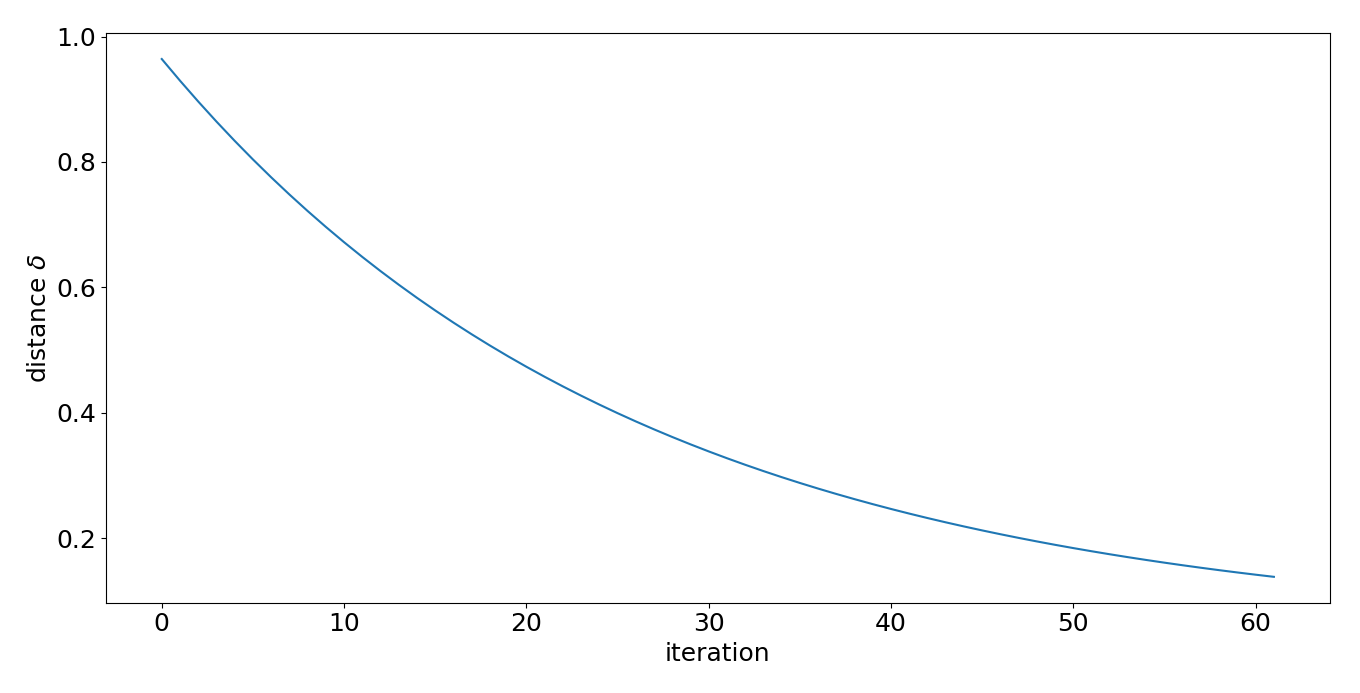
\includegraphics[width=1\linewidth]{./images/dist_plot.png}
    \caption{The distance between a robot and its kin after each step as it aggregates. We use $W=0.14$, $r_j=0.14$, $\Delta t=0.1$. In this example, aggregation took 60 iterations.}
    \label{fig:dist_plot}
  \end{figure}

  \begin{equation*} \label{eq:agg_final_result}
    \delta > \bigg(\frac{W}{4} + r_j\bigg)\tan\bigg(\frac{0.8\Delta t}{2W}\bigg)
  \end{equation*}

  We can now consider an example with the Khephera IV robot. The inner wheel distance for the Khephera IV is $W=$\SI{0.14}{\meter}, and in our simulations we use a time step of $\Delta t = 0.1s$. Therefore $\theta = 0.5714\;\text{rad}$ and $R=0.035$, and so aggregation is guaranteed when the following is true.

  \begin{equation} \label{eq:khephera_agg}
    \begin{split}
      \delta &> \bigg(0.035 + r_j\bigg)\tan\frac{0.5714}{2*0.14} \\
      \delta &> -1.96904 r_j - 0.06892
    \end{split}
  \end{equation}

   Note the largest possible value on the right hand side is achieved when $r_j=0$, at which point it equals $-0.06892$. However, since the distance between two robots $\delta$ must always be positive it will always be greater than $-0.06892$, we can say that it is guaranteed that Equation \ref{eq:khephera_agg} holds true for any $r_j$.

\section{Experimental Results}

  \subsection{Simulation Environment}

  We first extended the binary sensor presented in \cite{gauci_self-organized_2014} to be able to detect multiple types of robots. In our simulations, We use the range and bearing sensor with the FootBot robots and the ARGoS simulator, to detect whether a robot is in line of sight. If there is no robot, the sensor returns 0. If there is a robot, then the sensor returns 1 if the robot is kin (in the same class), and 2 if the robot is non-kin (in any other class).

  \subsection{Evolving Aggregation}

  \subsection{Evaluating the centroid-of-centroids cost function}

  When we implemented the centroid-of-centroids style cost function, we quickly found examples of configurations ranked in ways we did not like. One example is shown below in Figure \ref{fig:cost_function_fuckup}. The behavior that looks like aggregation was given lower cost of -8e9, versus the behavior that looks like segregation was given a cost of -5e9.

  \begin{figure}
    \centering
    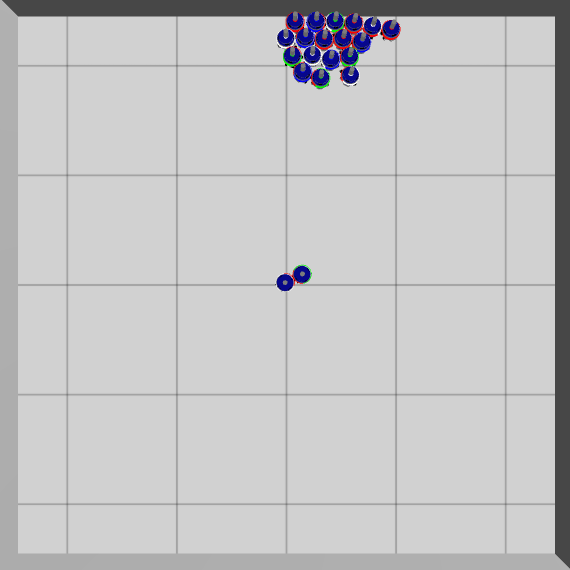
\includegraphics[width=0.49\linewidth]{./images/individual_0_gen_0.png}
    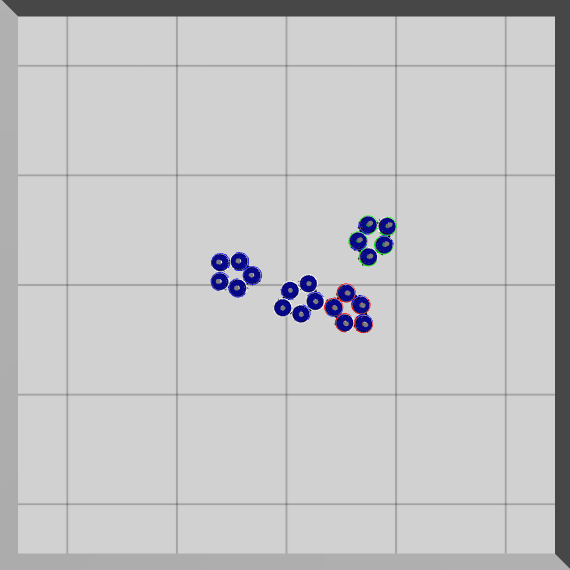
\includegraphics[width=0.49\linewidth]{./images/individual_0_gen_1_better.png}
    \caption{The left picture was given lower cost than the right, which is not desirable.}
    \label{fig:cost_function_fuckup}
  \end{figure}


  \subsection{Grid Search}

  \subsection{The effect of Beam Angle}

  \subsection{The effect of Beam Length}

\section{Future Work}
%  - consider the radius of the robot, track width, etc...

% consider more realistic applications i.e. different types of robots need to segregate, they may have different movement mechanisms e.g. some drive, some fly

\bibliography{RBE595.bib}
\bibliographystyle{unsrt}

\onecolumn
\appendix
%\section{Appendix}

\subsection{Proof of Theorem 1} \label{thm:1}

    \begin{align*}
      \lVert p_j - p'_i \rVert &< \lVert p_j - p_i \rVert \\
      \sqrt{(p_{j_x} - p'_{i_x})^2 + (p_{j_y} - p'_{i_y})^2} &< \sqrt{(p_{j_x} - p_{i_x})^2 + (p_{j_y} - p_{i_y})^2} \\
      (p_{j_x} - p'_{i_x})^2 + (p_{j_y} - p'_{i_y})^2 &< (p_{j_x} - p_{i_x})^2 + (p_{j_y} - p_{i_y})^2 \\
      (\delta - R\sin(\theta))^2 + (-(R+r_j) + R\cos(\theta))^2 &< \delta^2 + (-(R+r_j) + R)^2 \\
      (\delta - R\sin(\theta))^2 + (-(R+r_j) + R\cos(\theta))^2 &< \delta^2 + r_j^2 \\
      \delta^2 - 2R\delta\sin(\theta) + R^2\sin(\theta)^2 + (r_j + R(1 - \cos(\theta))^2 &< \delta^2 + r_j^2 \\
      \delta^2 - 2R\delta\sin(\theta) + R^2\sin(\theta)^2 + r_j^2 + 2Rr_j(1 - \cos(\theta)) + R^2(1 - \cos(\theta))^2 &< \delta^2 + r_j^2 \\
      \delta^2 - 2R\delta\sin(\theta) + R^2\sin(\theta)^2 + r_j^2 + 2Rr_j - 2Rr_j\cos(\theta) + R^2(1 - \cos(\theta))^2 &< \delta^2 + r_j^2 \\
      \delta^2 - 2R\delta\sin(\theta) + R^2\sin(\theta)^2 + r_j^2 + 2Rr_j - 2Rr_j\cos(\theta) + R^2(1 - 2\cos(\theta) + \cos(\theta)^2) &< \delta^2 + r_j^2 \\
      \delta^2 - 2R\delta\sin(\theta) + R^2\sin(\theta)^2 + r_j^2 + 2Rr_j - 2Rr_j\cos(\theta) + R^2 - 2R^2\cos(\theta) + R^2\cos(\theta)^2 &< \delta^2 + r_j^2 \\
      \delta^2 - 2R\delta\sin(\theta) + R^2(\sin(\theta)^2 + cos(\theta)^2) + r_j^2 + 2Rr_j - 2Rr_j\cos(\theta) + R^2 - 2R^2\cos(\theta) &< \delta^2 + r_j^2 \\
      \cancel{\delta^2} - 2R\delta\sin(\theta) + 2R^2 + \cancel{r_j^2} + 2Rr_j - 2Rr_j\cos(\theta) - 2R^2\cos(\theta) &< \cancel{\delta^2} + \cancel{r_j^2} \\
      -2R\delta\sin(\theta) + 2R^2 + 2Rr_j - 2Rr_j\cos(\theta) - 2R^2\cos(\theta) &< 0 \\
      -\delta\sin(\theta) + R + r_j - r_j\cos(\theta) - R\cos(\theta) &< 0 \qquad \text{assuming $R>0$}\\
      R + r_j - r_j\cos(\theta) - R\cos(\theta) &< \delta\sin(\theta) \\
      r_j(1 - \cos(\theta)) + R(1 - \cos(\theta)) &< \delta\sin(\theta) \\
      (r_j+R)(1 - \cos(\theta)) &< \delta\sin(\theta) \\
      (R+r_j)\bigg(\frac{1 - \cos(\theta)}{\sin(\theta)}\bigg) &< \delta \\
      (R+r_j)\tan{\frac{\theta}{2}}  &< \delta \\
    \end{align*}

\subsection{Proof of Theorem 2} \label{thm:2}

    \begin{align*}
      \Delta d &= d' - d \\
      &= \lVert p_j - p'_i \rVert - \lVert p_j - p_i \rVert \\
      &=\sqrt{(p_{j_x} - p'_{i_x})^2 + (p_{j_y} - p'_{i_y})^2} - \sqrt{(p_{j_x} - p_{i_x})^2 + (p_{j_y} - p_{i_y})^2} \\
      &=(p_{j_x} - p'_{i_x})^2 + (p_{j_y} - p'_{i_y})^2 - (p_{j_x} - p_{i_x})^2 + (p_{j_y} - p_{i_y})^2 \\
      &= (\delta - R\sin(\theta))^2 + (-(R+r_j) + R\cos(\theta))^2 - \delta^2 + (-(R+r_j) + R)^2 \\
      &= (\delta - R\sin(\theta))^2 + (-(R+r_j) + R\cos(\theta))^2 - \delta^2 + r_j^2 \\
      &= \delta^2 - 2R\delta\sin(\theta) + R^2\sin(\theta)^2 + (r_j + R(1 - \cos(\theta))^2 - \delta^2 + r_j^2 \\
      &= \delta^2 - 2R\delta\sin(\theta) + R^2\sin(\theta)^2 + r_j^2 + 2Rr_j(1 - \cos(\theta)) + R^2(1 - \cos(\theta))^2 - \delta^2 + r_j^2 \\
      &= \delta^2 - 2R\delta\sin(\theta) + R^2\sin(\theta)^2 + r_j^2 + 2Rr_j - 2Rr_j\cos(\theta) + R^2(1 - \cos(\theta))^2 - \delta^2 + r_j^2 \\
      &= \delta^2 - 2R\delta\sin(\theta) + R^2\sin(\theta)^2 + r_j^2 + 2Rr_j - 2Rr_j\cos(\theta) + R^2(1 - 2\cos(\theta) + \cos(\theta)^2) - \delta^2 + r_j^2 \\
      &= \delta^2 - 2R\delta\sin(\theta) + R^2\sin(\theta)^2 + r_j^2 + 2Rr_j - 2Rr_j\cos(\theta) + R^2 - 2R^2\cos(\theta) + R^2\cos(\theta)^2 - \delta^2 + r_j^2 \\
      &= \delta^2 - 2R\delta\sin(\theta) + R^2(\sin(\theta)^2 + cos(\theta)^2) + r_j^2 + 2Rr_j - 2Rr_j\cos(\theta) + R^2 - 2R^2\cos(\theta) - \delta^2 + r_j^2 \\
      &= \cancel{\delta^2} - 2R\delta\sin(\theta) + 2R^2 + \cancel{r_j^2} + 2Rr_j - 2Rr_j\cos(\theta) - 2R^2\cos(\theta) - \cancel{\delta^2} + \cancel{r_j^2} \\
      &= -2R\delta\sin(\theta) + 2R^2 + 2Rr_j - 2Rr_j\cos(\theta) - 2R^2\cos(\theta) \\
      &= 2R\big(-\delta\sin(\theta) + R + r_j - r_j\cos(\theta) - R\cos(\theta)\big) \\
      &= 2R\big((r_j + R)(1 - \cos(\theta))-\delta\sin(\theta)\big) \\
    \end{align*}

\end{document}
